\documentclass[12pt,a4paper]{article}
\usepackage[polish]{babel}
\usepackage[utf8]{inputenc}
\usepackage[T1]{fontenc}
\usepackage{pslatex} %z tym czcionka wygląda ładniej

\usepackage{xcolor}
\definecolor{CodeListingColor}{rgb}{0.95,0.95,0.95}
\usepackage{minted}

\usepackage{xpatch}
\xpretocmd{\inputminted}{\par\vspace{-1em}}{}{}
\xapptocmd{\inputminted}{\par\vspace{-1em}}{}{}

\usepackage{mathtools}
\DeclarePairedDelimiter\ceil{\lceil}{\rceil}
\DeclarePairedDelimiter\floor{\lfloor}{\rfloor}

\usepackage{amsfonts}
\usepackage{csvsimple}
%
\usepackage{adjustbox}

%%%%%%%%%%%%%%%%%%%%%%%%%%%%%%%%%%%%%%%
\usepackage{enumitem}
\makeatletter
\newcommand{\mtmathitem}{%
\xpatchcmd{\item}{\@inmatherr\item}{\relax\ifmmode$\fi}{}{\errmessage{Patching of \noexpand\item failed}}
\xapptocmd{\@item}{$}{}{\errmessage{appending to \noexpand\@item failed}}}
\makeatother

\newenvironment{mathitem}[1][]{%
\itemize[#1]\mtmathitem}{$\endlist}                    %$

\newenvironment{mathenum}[1][]{%
\enumerate[#1]\mtmathitem}{$\endlist}                  %$

\newenvironment{mathdesc}[1][]{%
\description[#1]\mtmathitem}{$\endlist}                %$
%%%%%%%%%%%%%%%%%%%%%%%%%%%%%%%%%%%%%%%

\usepackage[compact]{titlesec}
\titlespacing{\subsubsection}{0pt}{1em}{0em}
\setlength\parindent{0pt} %żeby wcięć przed akapitem nie było
\usepackage{parskip} %no need to use \\ to add empty line between paragraphs any more

%\author{
%  Ewa Fengler 132219
%  \and
%  Dariusz Grynia 132235
%  \and
%  gr. I1, wt. godz. 15.10, tyg. parzyste
%}
\date{}
\title{Przetwarzanie równoległe \\ \Large Projekt 2 CUDA}

\usepackage[a4paper, left=2.5cm, right=2.5cm, top=2.5cm, bottom=2.5cm, headsep=1.2cm]{geometry}
\usepackage[figurename=Rys.]{caption}
\usepackage{graphicx}
\usepackage[space]{grffile}
\usepackage{float}
%\usepackage{etoolbox}
%\makeatletter
%\patchcmd{\Ginclude@eps}{"#1"}{#1}{}{}
%\makeatother

\linespread{1.05}

\begin{document}
\maketitle
\thispagestyle{empty}


\section{Wstęp}

\subsection{Autorzy}
Ewa Fengler 132219\\
Dariusz Grynia 132235\\
grupa I1,\\
wtorki godz. 15.10,\\
tygodnie parzyste\\

\subsection{Adres kontaktowy}
dariusz.grynia@student.put.poznan.pl

\subsection{Temat zadania}
Ukrycie kosztów transferu danych w czasie obliczeń.

Porównanie wersji kodu:
\begin{itemize}
\item [3.] grid wieloblokowy, obliczenia przy wykorzystaniu pamięci współdzielonej bloku wątków
\item [5.] grid wieloblokowy, obliczenia przy wykorzystaniu pamięci współdzielonej bloku wątków, zrównoleglenie obliczeń i transferu danych między pamięciami: operacyjną procesora a globalną karty
\end{itemize}

\subsection{Opis wykorzystanej karty graficznej}

\begin{table}[H]
\centering
\def\arraystretch{1.5}
\begin{tabular}{|l|l|}
\hline
Model karty & GTX 260 \\
\hline
Compute Capability & 1,3 \\
\hline
Liczba multiprocesorów & 27 \\
\hline
Maksymalna liczba wątków we wiązce & 32 \\
\hline
Maksymalna liczba wiązek w ramach multiprocesora & 32 \\
\hline
Maksymalna liczba wątków w ramach multiprocesora & 1024 \\
\hline
Maksymalna liczba bloków wątków w ramach multiprocesora & 8 \\
\hline
Maksymalny rozmiar pamięci współdzielonej w ramach multiprocesora & 16384 B \\
\hline
Rozmiar bloku rejestrów & 16384 \\
\hline
Maksymalny rozmiar bloku wątków & 512 \\
\hline
\end{tabular}
\end{table}

\section{Analiza z przygotowania eksperymentu}

\subsection{Mnożenie macierzy z wykorzystaniem karty graficznej}

Mnożenie macierzy jest procesem kosztownym obliczeniowo i przez to czasochłonnym. Jednym z rozwiązań mających na celu skrócenie czasu przetwarzania jest podział pracy oraz zrównoleglenie obliczeń. W przypadku obliczeń z wykorzystaniem karty graficznej, w przeciwieństwie do obliczeń na procesorze wielordzeniowym ogólnego przeznaczenia, efektywne przetwarzanie wymaga dostosowania algorytmu mnożenia tak, aby wykorzystywał bardzo dużą liczbę wątków.

Mnożenie macierzy polega na obliczaniu jednej komórki macierzy wynikowej przez jeden wątek. Na pojedynczym multiprocesorze jednocześnie przetwarzane są wątki jednej wiązki. Wykonują one zawsze w danym momencie tę samą instrukcję, lecz na innych danych. Nie zawsze wątki są gotowe do obliczeń, np. w trakcie oczekiwania na dane. Wtedy sprzętowy moduł szeregujący wątki przełącza kontekst i następuje przetwarzanie gotowych wątków innej wiązki (z tego samego lub innego bloku wątków).

W trakcie całego procesu mnożenia macierzy, wykorzystywanych jest $n^2$ wątków (n -- jeden wymiar macierzy kwadratowej). Wątki są pogrupowane w bloki, te natomiast składają się na strukturę zwaną gridem. Taka organizacja umożliwia z jednej strony efektywne szeregowanie obliczeń wykonywanych na karcie graficznej, z drugiej strony pozwala programiście kontrolować na rzecz jakich danych wątki wykonują instrukcje, poprzez wykorzystanie identyfikatorów bloków oraz wątków wewnątrz bloku, np. do indeksowania tablic.

\subsection{Dostęp do pamięci}

Prędkość przetwarzania na procesorze ogólnego przeznaczenia w dużym stopniu zależała od efektywności dostępu do danych. Dostęp do pamięci operacyjnej cechował się stosunkowo dużym opóźnieniem, dlatego duże znaczenie miało efektywne wykorzystanie pamięci podręcznej.
W przypadku karty graficznej, dane mogą być przechowywane w stosunkowo powolnej pamięci globalnej. Opóźnienia są w tym przypadku bardzo znaczące i wynoszą 200 cykli procesora. W celu zwiększenia efektywności przetwarzania, należy wykorzystać odpowiednio dużą liczbę wątków, tak aby zawsze jakaś wiązka była gotowa do obliczeń, podczas gdy inne czekają na dane. Niestety z powodu ograniczeń na maksymalną liczbę wątków na multiprocesor, nadal nie jest możliwe zapewnienie ciągłości obliczeń.

W realizowanym temacie zostało wykorzystane inne podejście -- wykorzystanie pamięci współdzielonej, która jest znacznie szybsza od pamięci globalnej. Czas dostępu do danych znajdujących się w pamięci współdzielonej jest w przybliżeniu 100 razy krótszy niż w przypadku pamięci globalnej (pod warunkiem, że nie ma konfliktu dostępu do tych samych banków pamięci współdzielonej). Do danych znajdujących się w pamięci współdzielonej mają dostęp wszystkie wątki w ramach bloku. Zanim jednak będą mogły z nich korzystać, konieczne jest skopiowanie odpowiednich danych z pamięci globalnej do pamięci współdzielonej. W celu zwiększenia efektywności, dostępy do pamięci globalnej mogą być łączone w transakcje. Jednak aby było to możliwe, konieczne jest spełnienie następującego warunku: wątki w ramach pół-warpu muszą jednocześnie odwoływać się do sąsiednich adresów pamięci.


\subsection{Kod kernela}

% set options once for all listings
\setminted{
	frame=lines,
	framesep=2mm,
	baselinestretch=1.2,
	tabsize=2,
	bgcolor=CodeListingColor,
	%fontsize=\footnotesize,
	breaklines,
	linenos %Enables line numbers
}

\begin{listing}[ht!]
\inputminted{cuda}{listings/kernel.cu}
\caption{Kod kernela, obliczenia przy wykorzystaniu pamięci współdzielonej bloku wątków}
\label{lst:kernel}
\end{listing}

Kod źródłowy przedstawiony na listingu \ref{lst:kernel} to funkcja -- kernel, uruchamiany na karcie graficznej. Początkowe linie (4 - 13) służą wyznaczeniu przechowywanych w rejestrach wartości, wykorzystywanych dalej do indeksowania oraz sterowania pętlą. Następnie ma miejsce deklaracja tymczasowej zmiennej akumulującej obliczane iloczyny odpowiednich elementów macierzy. Pętla obejmujące linie 16 - 32 służy iteracji po kolejnych blokach macierzy A i B. Jeden blok wątków oblicza jeden blok macierzy wynikowej, jednak potrzebuje całego wiersza bloków macierzy A i całej kolumny bloków macierzy B, w celu wyznaczenia pełnego wyniku (analogicznie do zewnętrznych pętli metody 6-pętlowej dla CPU).

Linie 20-23 służą deklaracji oraz pobraniu danych z pamięci globalnej do pamięci współdzielonej. Wątki w ramach połowy warpu odwołują się do sąsiednich komórek macierzy (wartości \verb|tx| są kolejnymi liczbami), co pozwala na efektywny, łączony dostęp do pamięci globalnej.

W linii 24 ma miejsce synchronizacja wątków całego bloku. Gdyby w pamięci współdzielonej znajdował się tylko blok macierzy A, natomiast dane z macierzy B wątki odczytywałyby każdorazowo z pamięci globalnej, synchronizacja byłaby zbędna, ponieważ każda wiązka korzystałaby tylko z danych, które sama wcześniej pobrała. Wszystkie wątki wiązki wykonują w danym czasie tą samą instrukcję, kod nie zawiera żadnych rozgałęzień, a więc nie ma tutaj rozbieżności wątków. W przypadku omawianego kodu, w pamięci współdzielonej przechowywany jest także blok macierzy B.
Wątki danej wiązki odczytują kolejne wartości iterując po kolumnie macierzy B, a zatem korzystają również z danych, które są wczytywane przez pozostałe wiązki. Skutkiem tego synchronizacja jest konieczna, ponieważ wszystkie wiązki muszą uzupełnić blok macierzy B, zanim którakolwiek będzie mogła rozpocząć obliczenia. Wymagana synchronizacja do pewnego stopnia ogranicza wydajność, ponieważ nie ma możliwości jednoczesnego pobierania danych i wykonywania obliczeń przez różne wiązki bloku. Możliwa jest natomiast realizacja przetwarzania innego bloku wątków, przydzielonego na dany multiprocesor, w trakcie oczekiwania na dane przez tamten blok. Liczba bloków przypadających na multiprocesor jest jednak ograniczona, przez co karta graficzna może nie wykonywać obliczeń przez $100\%$ czasu.

Następnie w linii 29 ma miejsce faktyczne mnożenie macierzy. Jeden wątek oblicza jeden wynik, wykorzystując wiersz bloku macierzy A oraz kolumnę bloku macierzy B. Dyrektywa \verb|#pragma unroll| powoduje rozwinięcie pętli, co pozwala wyeliminować narzut wydajnościowy, który wynikałby ze sprawdzania warunku oraz inkrementacji zmiennej sterującej.

Po wykonaniu obliczeń, konieczna jest również synchronizacja, aby wątki należące do wiązek, które skończyły już obliczenia, nie mogły pobierać nowych danych do pamięci współdzielonej, w czasie kiedy inne wiązki jeszcze wykorzystują pobrany wcześniej fragment macierzy B do obliczeń.

Ostatecznie w linii 34 wynik przechowywany w zmiennej tymczasowej jest zapisywany macierzy C w pamięci globalnej pod odpowiednim indeksem. Tutaj również wątki odwołują się do kolejnych adresów, zatem możliwe jest połączenie danych zapisywanych przez wątki z połowy warpu w jedną transakcję.\\


{\footnotesize Przyjęto oznaczenie BS -- rozmiar bloku, które będzie dalej wykorzystywane w opisie instancji i wnioskach, poniżej oznacza ono że rysunek dotyczy bloku a nie całej macierzy}
\vspace{-0.3cm}
\begin{figure}[H]
  \centering
  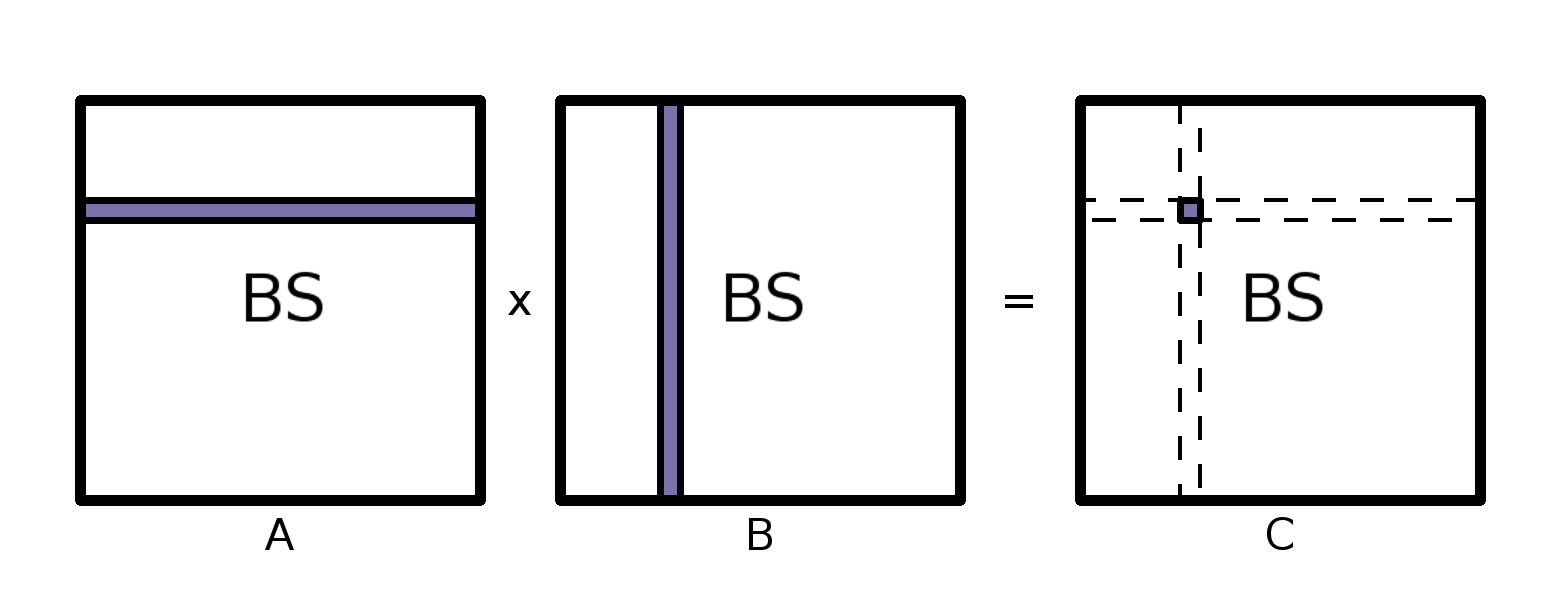
\includegraphics[width=\linewidth, trim={0 50px 0 90px}, clip=true]{images/2.jpg}
  \caption{Dane wykorzystywane przez jeden wątek w pętli wewnętrznej}
  \label{fig:matrix2}
\end{figure}
Pojedynczy wątek bloku iteruje po wierszu bloku macierzy A i kolumnie bloku macierzy B obliczając częściowy wynik przechowywany w rejestrze. Wartość jest zapisywana w rejestrze, i zostanie zapisana do pamięci globalnej po uzupełnieniu wyniku -- przejściu przez kolejne bloki macierzy). Trzeci rysunek pokazuje, który wynik jest wyznaczany.


\begin{figure}[H]
  \centering
  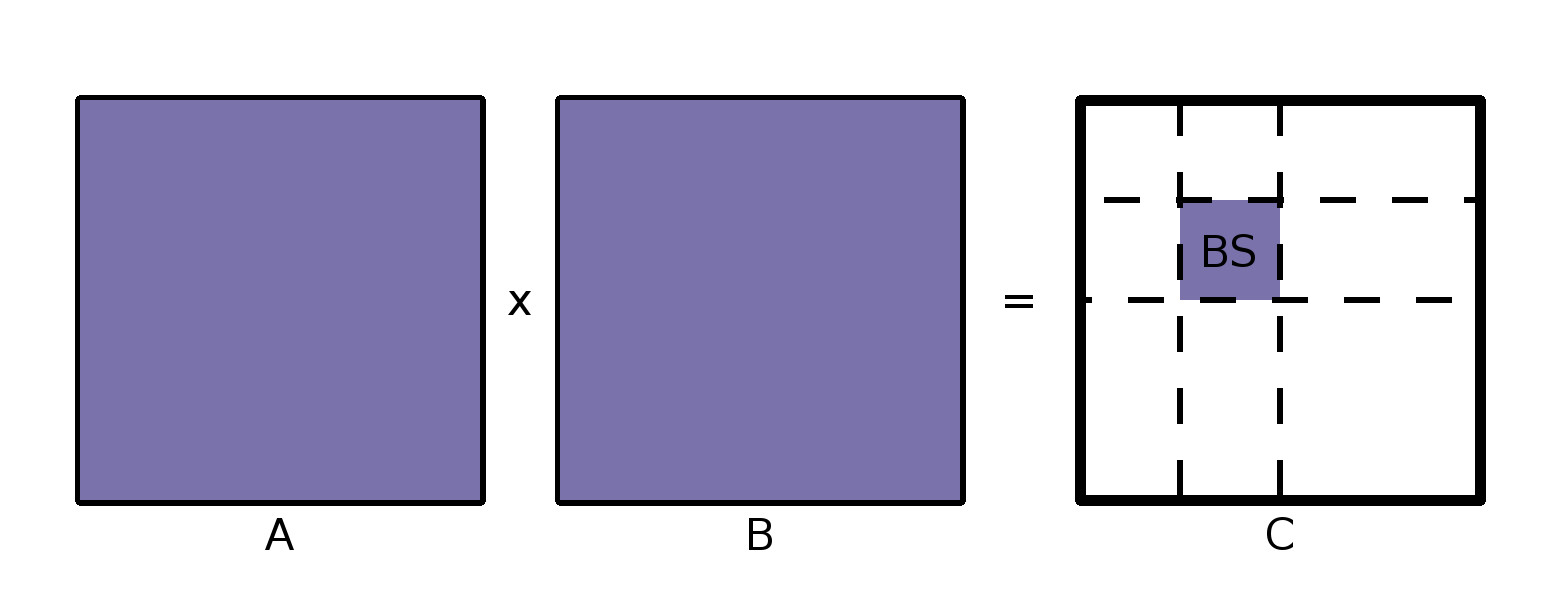
\includegraphics[width=\linewidth, trim={0 50px 0 90px}, clip=true]{images/1.jpg}
  \caption{Dane wykorzystywane przez blok wątków}
  \label{fig:matrix1}
\end{figure}

Jeden blok wątków wyznacza jeden blok macierzy wynikowej. W kolejnych iteracjach pętli zewnętrznej wykorzystuje kolejne bloki macierzy A oraz B.

\begin{figure}[H]
  \centering
  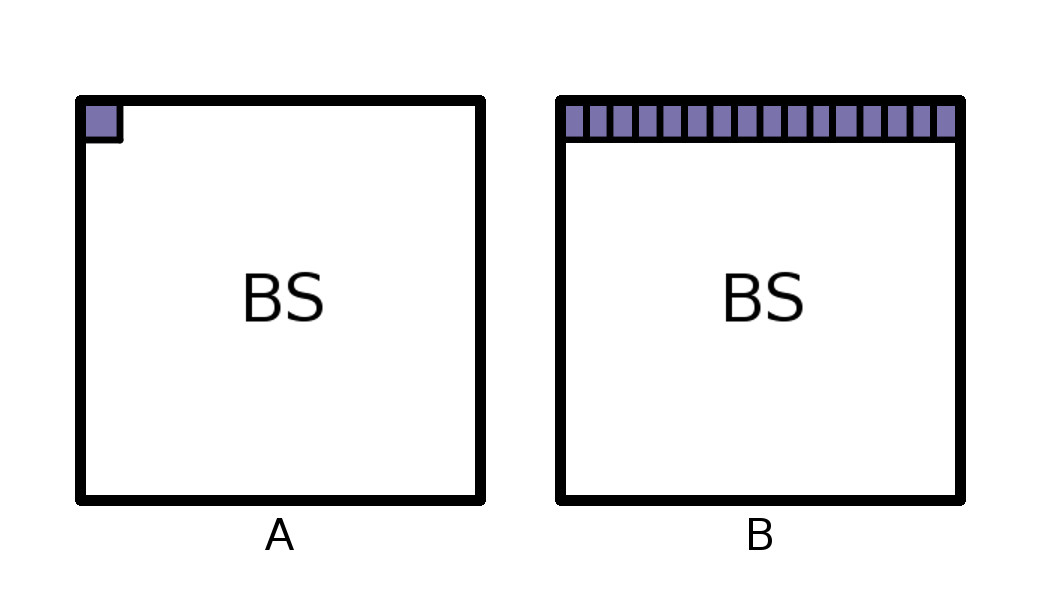
\includegraphics[width=0.66\linewidth, trim={0 50px 0 0px}, clip=true]{images/3.jpg}
  \caption{Wartości odczytywane przez pół warpu z pamięci współdzielonej: pole macierzy A i wiersz bloku macierzy B (ilustracja dla BS~=~16~x~16)}
  \label{fig:matrix2}
\end{figure}


\subsection{Wywołanie kernela}

\begin{listing}[H]
\inputminted{cuda}{listings/invocation_sync.cu}
\caption{Wywołanie kernela, wersja 3}
\label{lst:sync}
\end{listing}

Listing 2 przedstawia wywołanie kernela dla wersji trzeciej kodu. Zmienna \verb|nStreams| określa w tym przypadku ile macierzy będzie obliczanych, jednak przesyłanie macierzy wejściowych do pamięci karty graficznej, obliczenia oraz kopiowanie wyników do pamięci operacyjnej następują sekwencyjnie, po zakończeniu poprzedniej operacji. Do przechowywania wskaźników do segmentów pamięci zawierających dane wszystkich przetwarzanych macierzy wykorzystano wektory \verb|h_A, h_B, h_C|, zawierające wskaźniki do pamięci operacyjnej oraz \verb|d_A, d_B, d_C|, zawierające wskaźniki do danych w pamięci karty graficznej. Pamięć na karcie graficznej została wcześniej zaalokowana z wykorzystaniem funkcji \verb|cudaMalloc|. Poprawność wywołania wszystkich funkcji była sprawdzana, jednak, w celu zwiększenia czytelności, listingi 2 i 3 zawierają jedynie niezbędny do opisu koncepcji kod. Pełna wersja kodu, dołączona do sprawozdania, zawiera wszystkie szczegóły.

\begin{listing}[H]
\inputminted{cuda}{listings/invocation_async.cu}
\caption{Wywołanie kernela, wersja 5, zrównoleglenie obliczeń i transferu danych}
\label{lst:async}
\end{listing}

Na listingu 3 przedstawiono wywołanie kernela dla piątej wersji kodu, w której obliczenia na karcie graficznej zrównoleglono z przesyłaniem danych pomiędzy pamięcią karty a pamięcią operacyjną. W tym celu w liniach 1-4 zadeklarowano oraz zainicjowano strumienie, w liczbie równej liczbie obliczanych macierzy. Pamięć na karcie graficznej tutaj również zaalokowano wcześniej za pomocą funkcji \verb|cudaMalloc|, jednak w odróżnieniu od poprzedniej wersji, macierze znajdujące się w pamięci operacyjnej zaalokowano z wykorzystaniem funkcji \verb|cudaMallocHost|. Funkcja ta pozwala na alokację pamięci z wyłączonym stronicowaniem, co jest wymagane w przypadku asynchronicznych transferów wykonywanych przez funkcję \verb|cudaMemcpyAsync|. Kolejne pętle służą zakolejkowaniu operacji kopiowania danych do pamięci karty, wywołań kernela oraz kopiowania wyników do pamięci operacyjnej. Warto wspomnieć o każdorazowym przypisaniu danej operacji do strumienia, oraz o tym, że funkcje te są nieblokujące, oznaczają tylko zlecenie pewnej operacji, która jest wykonywana w tle. W ramach jednego strumienia operacje są oczywiście wykonywane sekwencyjnie, co gwarantuje, że dane wykorzystywane przez dany kernel zostaną przesłane przed jego uruchomieniem, natomiast wyniki zostaną przesłane do pamięci operacyjnej dopiero, gdy przetwarzanie kernela się zakończy. Zysk wynikający ze zrównoleglenia transferu danych będzie zatem widoczny w przypadku, gdy wykorzystany zostanie więcej niż jeden strumień.

W odróżnieniu od poprzedniej wersji, wykorzystano tutaj oddzielne pętle, służące do kolejkowania transferu danych oraz wywołań kernela. Ma to na celu zakolejkowanie najpierw wszystkich operacji przesyłania danych do karty, następnie wszystkich wywołań kerneli i na końcu wszystkich operacji kopiowania wyników obliczeń. W przypadku wykorzystania jednej pętli, wymienione operacje byłyby kolejkowane na przemian. Kolejność kolejkowania ma ogromne znaczenie w przypadku pracy z kartami graficznymi ze starszych generacji. W przypadku wykorzystywanej karty graficznej, GTX 260, compute capability 1.3, jedna jednostka kopiująca dane, operacje powinny być kolejkowane tak jak przedstawiono na listingu 3. W przypadku wykorzystania jednej pętli, mechanizm kolejkujący karty graficznej nie byłby w stanie zrównoleglić operacji.

\begin{figure}[H]
  \centering
  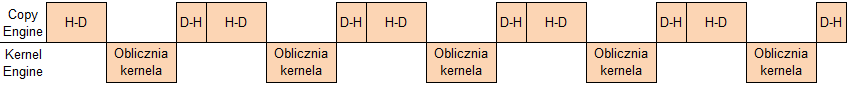
\includegraphics[width=\linewidth]{images/sync.png}
  \caption{Wersja 3 - kopiowanie na kartę graficzną, wykonywanie obliczeń i kopiowanie wyniku następują po sobie}
  \label{fig:seq}
\end{figure}

\begin{figure}[H]
  \centering
  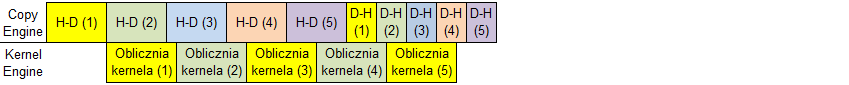
\includegraphics[width=\linewidth]{images/async.png}
  \caption{Wersja 5 - w trakcie obliczeń mogą być kopiowane dane kolejnych strumieni lub wyniki}
  \label{fig:async}
\end{figure}

Zupełnie inaczej sytuacja wygląda w przypadku kart graficznych z compute capability 2.0, kiedy dostępne są dwie jednostki kopiujące dane (jedna do pamięci globalnej karty, druga z pamięci karty graficznej do pamięci operacyjnej). W takim przypadku, oddzielne zakolejkowanie operacji w trzech pętlach umożliwiłoby jednoczesne kopiowanie danych do pamięci karty oraz wykonywanie obliczeń, jednak kopiowanie wyników następowałoby dopiero po skończeniu przetwarzania kernela ostatniego strumienia. Nie byłoby to optymalne, ponieważ druga jednostka kopiująca mogłaby kopiować dane strumienia, który zakończył już obliczenia w trakcie przetwarzania obliczeń następnego strumienia. Aby efektywnie wykorzystać możliwości takiej karty graficznej konieczne byłoby zastosowanie naprzemiennego kolejkowania operacji (jedna pętla).

Powyższe uwagi nie dotyczą nowszych kart graficznych, obsługujących co najmniej compute capability 3.5, w przypadku których kolejność zlecania operacji nie ma znaczenia, ponieważ system zarządzający potrafi uszeregować te operacje w optymalny sposób. Nowsze karty graficzne oferują także wiele innych usprawnień, m.in. zaawansowany mechanizm dostępu do pamięci globalnej, zmniejszający straty wydajności, w przypadkach gdzie dostęp do pamięci globalnej na kartach z compute capability nie mógł być łączony (z powodu nieodpowiedniego adresowania).


\section{Eksperyment pomiarowy}

\subsection{Instancje}

\subsubsection*{Rozmiar macierzy}
W zadaniu wykorzystano macierze kwadratowe o następujących rozmiarach (n - wielkość jednego wymiaru):
\begin{itemize}
\item n = 224
\item n = 1120
\item n = 864
\item n = 1728
\end{itemize}

\subsubsection*{Wielkość bloku wątków}

W celu zbadania wpływu rozmiaru bloku na czas obliczeń każda instancja została uruchomiona dla wielkości bloków:
\begin{itemize}
\item BS = 8 x 8
\item BS = 16 x 16
\end{itemize}

Wielkości instancji dobrano tak, aby zapewnić zrównoważone obciążenie karty graficznej. Rozmiar macierzy jest zawsze wielokrotnością rozmiaru bloku wątków, natomiast wielkość bloku wątków (64 lub 256) gwarantuje optymalny podział wątków na 32-wątkowe wiązki. Dzięki temu kod nie musi zawierać instrukcji warunkowych, sprawdzających czy dany wątek ma pracę. Wszystkie wątki wiązki zawsze wykonują w jednej chwili tę samą operację, a zatem rozbieżność przetwarzania wątków wiązki nie występuje.

W przypadku rozmiaru bloku BS~=~16~x~16, aby w pełni wykorzystać możliwości karty, instancja powinna mieć rozmiar, dla którego liczba wszystkich bloków będzie wielokrotnością liczby 108. Wynika to z faktu, że jeden multiprocesor może przetwarzać współbieżnie (przełączając wiązki) 1024 wątki, co daje cztery 256-wątkowe bloki na każdy z 27 multiprocesorów. Instancja  n~=~224, BS~=~16~x~16 zostanie podzielona na 196 bloków, dlatego też, w pewnym momencie obliczeń, niektóre mutliprocesory nie będą w pełni zajęte. Liczba bloków równa 216 zapewniłaby optymalne wykorzystanie zasobów karty, jednak nie da się stworzyć macierzy kwadratowej, która dzieliłaby się na tyle bloków. Można zatem przyjąć, że średnie teoretyczne wykorzystanie zasobów karty graficznej wynosi $196 / 216 \approx 91\% $. Analogicznie dla instancji  n~=~1120, BS~=~16~x~16, uzyskamy wartość $4900 / 4968 \approx 99\% $

W przypadku rozmiaru bloku  BS~=~8~x~8, liczba bloków przydzielonych na jeden multiprocesor powinna wynosić 16. Niestety, dla compute capability 1.3 maksymalna liczba bloków aktywnych jednocześnie na multiprocesorze wynosi 8. Dlatego też multiprocesor będzie przetwarzał maksymalnie 512 wątków, przez co jego zajętość wyniesie maksymalnie $50\%$.  Uwzględniając fakt, że liczba bloków nie jest równa wielokrotności 216 (8 bloków na każdy z 27 multiprocesorów), średnie teoretyczne wykorzystanie zasobów całej karty wyniesie ok. $45\%$ dla instancji n~=~224 oraz n~=~1120.

Eksperyment nie obejmuje obliczeń z wykorzystaniem bloków wątków o wymiarach 32~x~32, ponieważ wykorzystana karta graficzna nie pozwala na stworzenie bloków zawierających więcej niż 512 wątków.


\subsubsection*{Liczba obliczanych macierzy}

Skrócenie czasu przetwarzania w wersji 5 (zrównoleglenie obliczeń i transferu danych) jest możliwe, jeśli wykorzystamy więcej niż jeden strumień. Eksperyment przeprowadzono dla 1, 5 i 10 obliczanych macierzy. W przypadku obliczania tylko jednej macierzy, należy spodziewać się braku skrócenia czasu przetwarzania w stosunku do wersji 3 kodu.

\subsection{Mierzone parametry}

Czas przetwarzania każdej instancji był mierzony w kodzie, za pomocą zdarzeń start i stop (na podstawie przykładowych kodów NVIDII). Obejmował on czas kopiowania danych na kartę graficzną, czas przetwarzania kerneli oraz czas kopiowania wyników do pamięci operacyjnej.

Za pomocą programu NVIDIA Visual Profiler dokonano pomiaru zdarzeń związanych z dostępem do pamięci. Metryki potrzebne do zbadania efektywności to: 
\begin{itemize}
\item \verb|gld 32B| -- liczba 32 bajtowych transakcji pobierania danych z pamięci globalnej,
\item \verb|gld 64B| -- liczba 64 bajtowych transakcji pobierania danych z pamięci globalnej,
\item \verb|gst 32B| -- licznik 32 bajtowych transakcji zapisu danych do pamięci globalnej, każda transakcja powoduje inkrementację licznika o 2,
\item \verb|gst 64B| -- licznik 64 bajtowych transakcji zapisu danych do pamięci globalnej, każda transakcja powoduje inkrementację licznika o 4.
\end{itemize}

Ponadto w celu obliczenia wartości miar \verb|gld efficiency| oraz \verb|gst efficiency| potrzebne są także liczniki  \verb|gld request| oraz  \verb|gst request|. Niestety z niewyjaśnionych przyczyn program NVIDIA Visual Profiler nie był w stanie zebrać tych  miar (wartości dla wszystkich testowanych instancji były równe 0). W przypadku realizowanego zadania miary te nie są jednak kluczowe, ponieważ celem było zbadanie przyspieszenia przetwarzania dzięki zrównolegleniu obliczeń oraz transferów między pamięcią operacyjną a globalną karty.


\subsection{Wyniki eksperymentu}

Dane zebrane podczas eksperymentu zostały dołączone do sprawozdania. Są to surowe dane z profilera, obliczone miary oraz zrzuty ekranu, które dobrze obrazują sposób przetwarzania i zyski z ukrycia kosztów transferu danych. Przyjęto następujące nazewnictwo zrzutów ekranu ,,N BS Wersja Lm'', przykładowo plik ,,1728 16 3 5.png'' oznacza instancję o rozmierze macierzy 1728~x~1728, rozmiarze bloku 16~x~16, wykorzystanie kodu w wersji 3 oraz obliczaniu 5 macierzy.

Warto zwrócić uwagę na wskaźnik \verb|warp serialize| (dokładne wartości w załączonym arkuszu). Określa on liczbę wiązek, dla których dostęp do pamięci współdzielonej musiał odbywać się sekwencyjnie z powodu konfliktu w dostępie do banków pamięci. W przypadku omawianego kodu, konflikt nigdy nie powinien występować, zarówno w przypadku wykorzystania bloków 16~x~16 jaki i 8~x~8. Wartość tego wskaźnika jest jednak niezerowa w przypadku wszystkich instancji, gdzie BS~=~8~x~8. Trudno wyjaśnić co wpłynęło na taki wynik, być może wątki w przypadku instancji z tym rozmiarem bloku były szeregowane w inny sposób, przez co konflikty w dostępie były \texttt{możliwe}.

\subsection{Wzory}

Prędkość przetwarzania
\begin{equation}
PP = \frac{Z}{T} = \frac{2 \cdot n^3}{T} \; \in \; \mathbb{R}_+
\end{equation}

Przyspieszenie przetwarzania wersji 5 kodu (ukrywanie kosztów transferu w czasie obliczeń) do wersji 3
\begin{equation}
P_{w5} = \frac{T_{w5}}{T_{w3}} \cdot 100\% \; \in \; \mathbb{R}_+
\end{equation}

Przyspieszenie w stosunku do obliczeń sekwencyjnych na CPU metodą IKJ
\begin{equation}
P_{GPU} = \frac{T_{GPU}}{T_{CPU}} \cdot 100\% \; \in \; \mathbb{R}_+
\end{equation}

Sposób obliczenia zajętości multiprocesora został omówiony w punkcie 3.1, natomiast sposób wyznaczenia CGMA we wnioskach.

\subsection{Wyniki}

Poniższa tabela oraz wykresy obrazują efektywność przetwarzania poszczególnych instancji. Pełne, pogrupowane dane oraz wykresy znajdują się również w załączonym arkuszu.

\begin{table}[H]
\centering
\def\arraystretch{1.05}
\begin{adjustbox}{totalheight=\textheight-\baselineskip}
\begin{tabular}{|c|c|c|c|c|c|c|}
\hline
N	&	BS	&	Wersja kodu	&	Lm	&	Czas [ms]	&	$PP$ [GFLOPS]	&	$P_{GPU}$	\\ \hline
224	&	16	&	5	&	10	&	4.49968	&	49.96	&	17.84	\\ \hline
224	&	16	&	3	&	10	&	6.58928	&	34.11	&	12.18	\\ \hline
224	&	8	&	5	&	10	&	4.95914	&	45.33	&	16.19	\\ \hline
224	&	8	&	3	&	10	&	9.0527	&	24.83	&	8.87	\\ \hline
224	&	16	&	5	&	5	&	2.87206	&	39.13	&	14.67	\\ \hline
224	&	16	&	3	&	5	&	3.47869	&	32.31	&	12.11	\\ \hline
224	&	8	&	5	&	5	&	3.99331	&	28.15	&	10.55	\\ \hline
224	&	8	&	3	&	5	&	4.14125	&	27.14	&	10.18	\\ \hline
224	&	16	&	5	&	1	&	1.72758	&	13.01	&	5.23	\\ \hline
224	&	16	&	3	&	1	&	0.820768	&	27.39	&	11.01	\\ \hline
224	&	8	&	5	&	1	&	1.7937	&	12.53	&	5.04	\\ \hline
224	&	8	&	3	&	1	&	0.872416	&	25.77	&	10.36	\\ \hline
1120	&	16	&	5	&	10	&	148.783	&	188.86	&	45.37	\\ \hline
1120	&	16	&	3	&	10	&	232.467	&	120.87	&	29.04	\\ \hline
1120	&	8	&	5	&	10	&	277.647	&	101.2	&	24.31	\\ \hline
1120	&	8	&	3	&	10	&	358.398	&	78.4	&	18.84	\\ \hline
1120	&	16	&	5	&	5	&	76.5913	&	183.43	&	44.34	\\ \hline
1120	&	16	&	3	&	5	&	115.322	&	121.83	&	29.45	\\ \hline
1120	&	8	&	5	&	5	&	144.852	&	96.99	&	23.45	\\ \hline
1120	&	8	&	3	&	5	&	177.629	&	79.09	&	19.12	\\ \hline
1120	&	16	&	5	&	1	&	18.5323	&	151.62	&	37.09	\\ \hline
1120	&	16	&	3	&	1	&	22.7764	&	123.37	&	30.18	\\ \hline
1120	&	8	&	5	&	1	&	31.626	&	88.85	&	21.74	\\ \hline
1120	&	8	&	3	&	1	&	36.3668	&	77.26	&	18.9	\\ \hline
864	&	16	&	5	&	10	&	36.3386	&	354.98	&	75.49	\\ \hline
864	&	16	&	3	&	10	&	59.0637	&	218.4	&	46.44	\\ \hline
864	&	8	&	5	&	10	&	65.9215	&	195.68	&	41.61	\\ \hline
864	&	8	&	3	&	10	&	88.1335	&	146.36	&	31.12	\\ \hline
864	&	16	&	5	&	5	&	9.89984	&	651.5	&	140.53	\\ \hline
864	&	16	&	3	&	5	&	12.0329	&	536.01	&	115.62	\\ \hline
864	&	8	&	5	&	5	&	15.7338	&	409.93	&	88.42	\\ \hline
864	&	8	&	3	&	5	&	17.9046	&	360.23	&	77.7	\\ \hline
864	&	16	&	5	&	1	&	69.9345	&	18.45	&	4.02	\\ \hline
864	&	16	&	3	&	1	&	120.85	&	10.67	&	2.33	\\ \hline
864	&	8	&	5	&	1	&	129.023	&	10	&	2.18	\\ \hline
864	&	8	&	3	&	1	&	176.783	&	7.3	&	1.59	\\ \hline
1728	&	16	&	5	&	10	&	538.58	&	191.61	&	75.36	\\ \hline
1728	&	16	&	3	&	10	&	721.525	&	143.02	&	56.25	\\ \hline
1728	&	8	&	5	&	10	&	1873.81	&	55.07	&	21.66	\\ \hline
1728	&	8	&	3	&	10	&	2056.47	&	50.18	&	19.74	\\ \hline
1728	&	16	&	5	&	5	&	273.57	&	188.61	&	74.37	\\ \hline
1728	&	16	&	3	&	5	&	360.715	&	143.04	&	56.4	\\ \hline
1728	&	8	&	5	&	5	&	941.951	&	54.78	&	21.6	\\ \hline
1728	&	8	&	3	&	5	&	1024.74	&	50.35	&	19.85	\\ \hline
1728	&	16	&	5	&	1	&	61.2197	&	168.57	&	66.52	\\ \hline
1728	&	16	&	3	&	1	&	72.2033	&	142.92	&	56.4	\\ \hline
1728	&	8	&	5	&	1	&	191.03	&	54.02	&	21.32	\\ \hline
1728	&	8	&	3	&	1	&	207.458	&	49.74	&	19.63	\\ \hline
\end{tabular}
\end{adjustbox}
\caption{Prędkość przetwarzania oraz przyspieszenie względem CPU}
\label{table:all}
\end{table}


Poniższe wykresy przedstawiają stosunek czasu przetwarzania wersji 5 do wersji 3 kodu.
\begin{figure}[H]
  \centering
    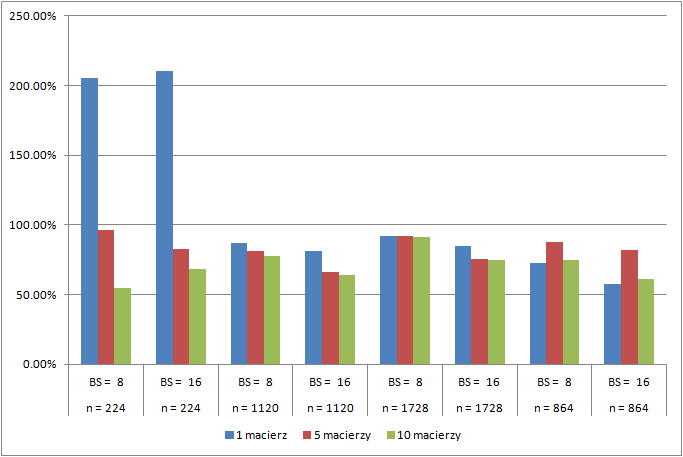
\includegraphics[width=0.95\textwidth]{charts/Lm.png}
    \caption{Wpływ liczby obliczanych na przyspieszenie}
    \label{chart:Lm}
\end{figure}

\begin{figure}[H]
  \centering
    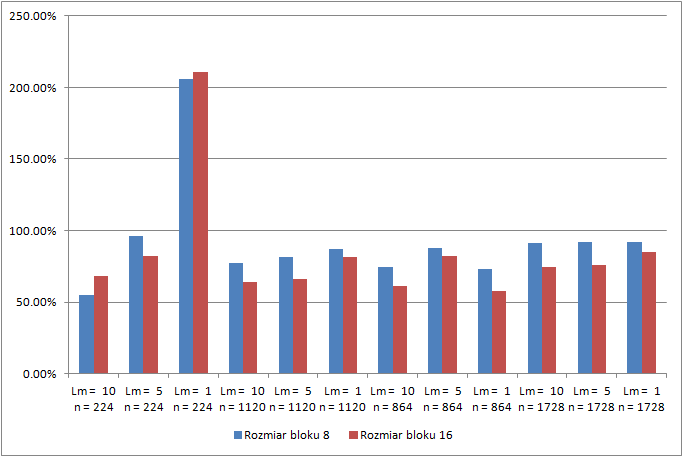
\includegraphics[width=0.95\textwidth]{charts/BS.png}
    \caption{Wpływ wielkości bloku wątków na przyspieszenie}
    \label{chart:BS}
\end{figure}

\begin{figure}[H]
  \centering
    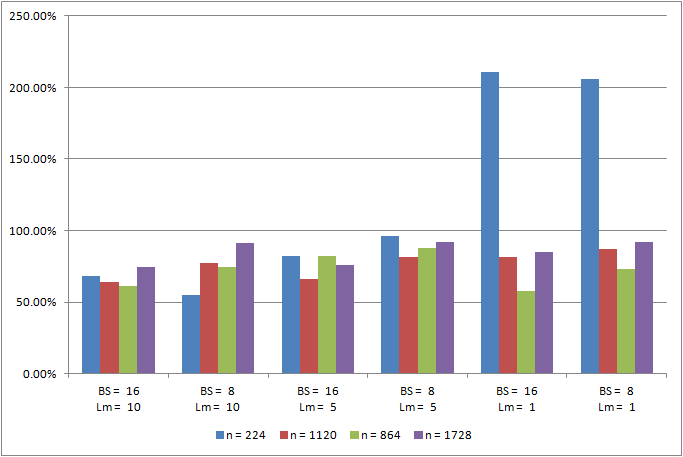
\includegraphics[width=0.95\textwidth]{charts/MatrixSize.png}
    \caption{Wpływ rozmiaru pojedynczej macierzy na przyspieszenie}
    \label{chart:MatrixSize}
\end{figure}


\section{Wnioski}

\subsection{Dostęp do pamięci globalnej}

Wartości miar \verb|gld| oraz \verb|gst| zebranych przez NVIDIA Visual Profiler wskazują, że zgodnie z przeprowadzoną wcześniej analizą, wszystkie dostępy do pamięci globalnej były łączone w transakcje. W przypadku bloków o rozmiarze 16~x~16 wszystkie dostępy (pobieranie danych oraz zapis wyników) były przeprowadzane w transakcjach 64 bajtowych (tylko wartości \verb|gld 64B| oraz \verb|gst 64B| są niezerowe). Oznacza to, że dostęp do pamięci globalnej był przeprowadzany w optymalny sposób (64B to 16 zmiennych typu float, czyli zawsze dostępy połowy wiązki były łączone w jedną transakcję).

W przypadku wszystkich instancji gdzie bloki wątków miały rozmiar 8~x~8, tylko wartości \verb|gld 32B| oraz \verb|gst 32B| miały wartości niezerowe. Oznacza to, że żądania każdych ośmiu wątków wiązki były łączone w jedną transakcje. Jest to konsekwencją tego, że wątki jednego bloku pobierają lub zapisują dane do fragmentu 8~x~8 pełnej macierzy. Oznacza to, że tylko 8 komórek ma sąsiednie adresy (wiersz bloku), natomiast kolejne 8 wątków pobiera oddalone dane z następnego wiersza macierzy. Z tego powodu nie jest możliwe łączenie dostępów w transakcje 64 bajtowe.

Dostęp do pamięci w przypadku wykorzystania bloków wątków 8~x~8 wciąż jest bardziej efektywny, niż w przypadku kiedy łączenie nie byłoby w ogóle możliwe, jednak dla bloków 16~x~16 można uzyskać optymalną efektywność dostępów do pamięci globalnej. Dodatkowo, wykorzystanie mniejszych bloków pozwala osiągnąć zajętość multiprocesora równą maksymalnie 50\%. Z tego powodu, w przypadku chęci maksymalizacji efektywności przetwarzania wykorzystanie mniejszych bloków nie ma sensu.

\subsection{Zajętość multiprocesora}

W celu zapewnienia optymalnej efektywności przetwarzania, należy maksymalizować zajętość wszystkich multiprocesorów karty. Dla instancji n~=~224 oraz n~=~1120 oraz obu rozważanych rozmiarów bloku wątków analiza zajętości została przeprowadzona już w punkcie 3.2. Dwie pozostałe instancje n~=~864 oraz n~=~1728, zostały wybrane, ponieważ umożliwiają osiągnięcie  100\% teoretycznej zajętości wszystkich multiprocesorów, w przypadku bloków 16~x~16. W przypadku mniejszych bloków, zajętość procesorów osiągnie 50\%, ograniczeniem jest tutaj limit 8 bloków na multiprocesor.

W przypadku każdej testowanej instancji żądania zasobowe dotyczące liczby rejestrów oraz pamięci współdzielonej były na tyle małe, że nie stanowiły ograniczenia dla zajętości multiprocesorów. Liczba wykorzystywanych przez wątek rejestrów była zawsze równa 13, co pokrywa się z liczbą zmiennych lokalnych w kodzie kernela, natomiast rozmiar wykorzystanej pamięci współdzielonej przez blok był równy 548 B dla BS~=~8~x~8 oraz 2084 B dla BS~=~16~x~16. W obu przypadkach wartość ta była większa o 36 B od spodziewanej, przypuszczalnie więc karta graficzna zawsze wykorzystuje niewielką ilość pamięci współdzielonej do innych celów.

\subsection{CGMA}

CGMA (Compute to Global Memory Access ratio) jest współczynnikiem określającym intensywność obliczeń, to znaczy ile operacji arytmetycznych (w przypadku mnożenia macierzy będą to operacje dodawania i mnożenia) przypada na dostęp do danych w pamięci globalnej. W przypadku mnożenia macierzy z wykorzystaniem pamięci współdzielonej do przechowywania wielokrotnie wykorzystywanych bloków macierzy A i B, CGMA będzie równe $2 \cdot \text{BS} / 3$. Wynika to z faktu, że każdy wątek bloku pobiera do pamięci współdzielonej po jednej wartości z macierzy A oraz B. Następnie dany wątek w pętli wewnętrznej wykorzystuje jeden wiersz bloku macierzy A oraz jedną kolumnę bloku macierzy B, a zatem wykonuje dwie operacje arytmetyczne BS razy, samemu pobierając wcześniej z pamięci globalnej tylko 2 wartości. Ostatecznie każdy wątek zapisuje jedną wartość (wynik) do pamięci globalnej, stąd łącznie wartość mianownika wynosi 3 (2 odczyty, 1 zapis).

\subsection{Skrócenie czasu przetwarzania wersji 5 kodu}

\subsubsection*{Wpływ liczby obliczanych macierzy}

W przypadku obliczania tylko jednej macierzy spodziewanym wynikiem jest brak przyspieszenia, ponieważ nie da się zrównoleglić przesyłania danych i obliczeń. Czas przetwarzania wersji 5 kodu był jednak prawie zawsze krótszy. Jest to spowodowane różnym sposobem alokacji pamięci hosta. Wersja 5 wymagała pamięci z wyłączonym stronicowaniem. Okazuje się jednak, że transfer danych zaalokowanych w ten sposób zwykle jest nieco szybszy, niż w przypadku pamięci stronicowanej.

W celu określenia zysku wynikającego wyłącznie ze zrównoleglenia transferu danych i obliczeń, dobrze byłoby przeprowadzić dodatkowy eksperyment dla 3 wersji kodu również z wykorzystaniem pamięci z wyłączonym stronicowaniem. Podczas analizy wpływu innych parametrów na skrócenie czasu przetwarzania nie należy zatem brać pod uwagę instancji, gdzie obliczana była tylko jedna macierz. Wykres \ref{chart:Lm} pokazuje, że zwykle większa liczba obliczanych powodowała większe skrócenie czasu przetwarzania. Ciekawy jest również fakt, że w przypadku bardzo małych macierzy (n~=~224), czas przetwarzania piątej wersji kodu był dłuższy. Pełne wyniki, oraz załączone zrzuty ekrany z profilera, pokazują, że dla tych instancji, czas kopiowania pamięci niestronicowanej był jednak nieco dłuższy, ponadto czas obliczeń dla małych instancji jest krótki, (w porównaniu do stosunku czasu przetwarzania a czasu kopiowania danych dla większych macierzy), co spowodowało spadek prędkości przetwarzania.

Pamięć niestronicowana ma wiele zalet, pozwala na wykorzystanie strumieni do zrównoleglenia transferu danych oraz obliczeń, a także cechuje się nieco większą szybkością kopiowania danych. Pamięć ta nie powinna być jednak nadużywana. Po pierwsze pamięć niestronicowana jest zasobem ograniczonym. Może się okazać, że alokacja większej ilości takiej pamięci zakończy się niepowodzeniem, podczas gdy można jeszcze alokować pamięć w zwykły sposób (stronicowaną). Po drugie, zmniejszanie ilości dostępnej fizycznej pamięci dla systemu operacyjnego może wpłynąć na ogólny spadek wydajności systemu obliczeniowego. Ponadto, alokacja pamięci niestronicowanej, jest zazwyczaj bardziej wymagająca dla systemu zarządzania pamięcią. Pomiar czasu na potrzeby eksperymentu nie obejmował czasu potrzebnego na alokację pamięci, jednak w praktycznych zastosowaniach, jeśli wykorzystanie pamięci niestronicowanej nie jest konieczne, należy najpierw sprawdzić, które rozwiązanie okaże się bardziej efektywne.

\subsubsection*{Wpływ wielkości bloku wątków}

Zgodnie z wykresem \ref{chart:BS} wykorzystanie większego rozmiaru bloku przekłada się na większy zysk ze zrównoleglenia obliczeń i przesyłania danych. Jest to zgodne z oczekiwaniami, ponieważ czas przetwarzania obliczeń w przypadku bloków 8~x~8 był zawsze dłuższy (z powodu małej zajętości multiprocesorów). Z tego powodu koszt przesyłania danych stanowi większy procent łącznego czasu przetwarzania dla BS~=~16~x~16. Ukrycie kosztów transferu danych przynosi zatem większe zyski.

\subsubsection*{Wpływ wielkości pojedynczej macierzy}

Analizując wykres \ref{chart:MatrixSize} trudno dostrzec wyraźną zależność skrócenia czasu od rozmiaru macierzy. Biorąc pod uwagę fakt, że koszt przesyłania danych stanowi większy procent czasu w przypadku mniejszych instancji (trzeba przesłać łącznie $3n^2$ danych, natomiast złożoność obliczeniowa wynosi $2n^3$, należy się spodziewać większych zysków w przypadku mniejszych macierzy. Wyniki dla instancji n~=~864 oraz n~=~1728 potwierdzają te przypuszczenia. Dwie pozostałe instancje nie potwierdzają tej tezy, jednak w tym przypadku wyniki są zaburzone przez fakt, że charakteryzowały się one różną zajętością multiprocesorów. Szczególny przypadek stanowi instancja n~=~224, gdzie obliczenia czasem trwały krócej niż przesyłanie danych (sytuację tą dobrze obrazują dołączone zrzuty ekranu). Powód wydłużenia czasu przetwarzania wersji 5 kodu dla instancji n~=~224, Lm~=~1 został omówiony wcześniej, przy okazji analizy wpływu obliczanych macierzy.


\subsection{Przyspieszenie przetwarzania względem CPU}

Wyniki zebrane w kolumnie $P_{GPU}$ tabeli \ref{table:all} pokazują, że mnożenie macierzy na karcie graficznej trwało krócej dla każdej testowanej instancji. Mnożenie macierzy jest świetnym przykładem problemu obliczeniowego, gdzie wykorzystanie karty graficznej, umożliwiającej współbieżne przetwarzanie bardzo dużej liczby wątków, przynosi znaczące zyski. Znaczące zyski czasowe przynosi optymalizacja algorytmu za pomocą takich technik jak wykorzystanie pamięci współdzielonej (dzięki lokalności czasowej dostępów do danych -- wielokrotne wykorzystanie danych raz pobranych z pamięci globalnej). Jeśli problem pozwala w łatwy sposób rozdzielić obliczenia na części składowe lub obliczenia polegają na przetwarzaniu wielu niezależnych danych, to warto również wykorzystać możliwość zrównoleglenia transferu danych z obliczeniami.

Wartość miary przyspieszenia różni się dla poszczególnych instancji. Ogólna zależność jaką można zauważyć, to większe przyspieszenie w przypadku instancji w pełni wykorzystującej możliwości karty (pełne obciążenie wszystkich multiprocesorów) i mniejsze dla małych instancji oraz bloków o rozmiarze 8~x~8. Należy również zwrócić uwagę na to, że nie wszystkie instancje były przetwarzane na procesorze z tą samą prędkością.


\end{document}